The distribution of Part-of-Speech tags (NN, NNP, NNS, VB variants, JJ, IN being most frequent) confirmed that the email text follows typical English grammatical structures.

\begin{figure}[H]
    \centering
    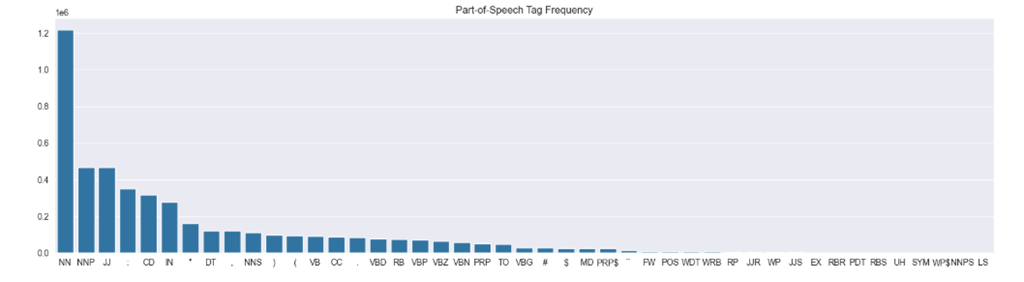
\includegraphics[width=\linewidth]{images/pos-tag-frequency}
    \caption{Bar Chart for POS Tag Frequency}
    \label{fig:pos-tag-frequency}
\end{figure}

Observations:
\begin{itemize}
    \item Nouns are highly frequent: The tags ``NN'' (singular nouns) and ``NNP'' (proper nouns) have the tallest bars,indicating they are the most frequent part-of-speech tags in this text.
    \item Adjectives and Prepositions/Conjunctions are also common: ``JJ'' (adjectives) and ``IN'' (prepositions/subordinating conjunctions) show relatively high frequencies as well.
    \item Verbs have varied frequencies: Different verb forms (``VB'', ``VBP'', ``VBZ'',``VBN'', ``VBG'') show varying levels of frequency, with the base form (``VB'') and non-3rd person singular present (``VBP'') being more common than others.
    \item Determiners are significant: ``DT'' (determiners like ``the'', ``a'', ``an'') also appear frequently.
    \item Other parts of speech are less frequent: Tags like adverbs (``RB''), pronouns (``PRP'', ``PRP\$''), modals (``MD''), coordinating conjunctions (``CC''), and various wh-words (``WDT'', ``WRB'', ``WP'', ``WP\$'') have noticeably lower frequencies compared to nouns and adjectives.
    \item Symbols and foreign words are rare: Tags like ``\$'' (dollar sign), ``FW'' (foreign word), and other symbols (``SYM'') have very short bars, indicating they are not common in this text.
\end{itemize}